% One-page size proof; this is not a submitted manuscript.
\documentclass[UTF8,a4paper,zihao=-4]{ctexart}
\usepackage[margin=2.3cm]{geometry}
\usepackage{graphicx,amsmath,lmodern,caption,float}
\captionsetup{font=small,labelsep=quad}
\pagestyle{empty}
\begin{document}
在问题二中，附录3给出的热物性随局部含水率变化，而水分扩散系数同时依赖局部温度和含水率。因此，两场在当前状态下相互影响，需要联合求解。图\ref{fig:mechanism}将内部控制方程、径向几何与侧表面交换对应起来；问题三沿用这组物理关系，并进一步确定全域含水率达标时刻。

\begin{figure}[H]
\centering
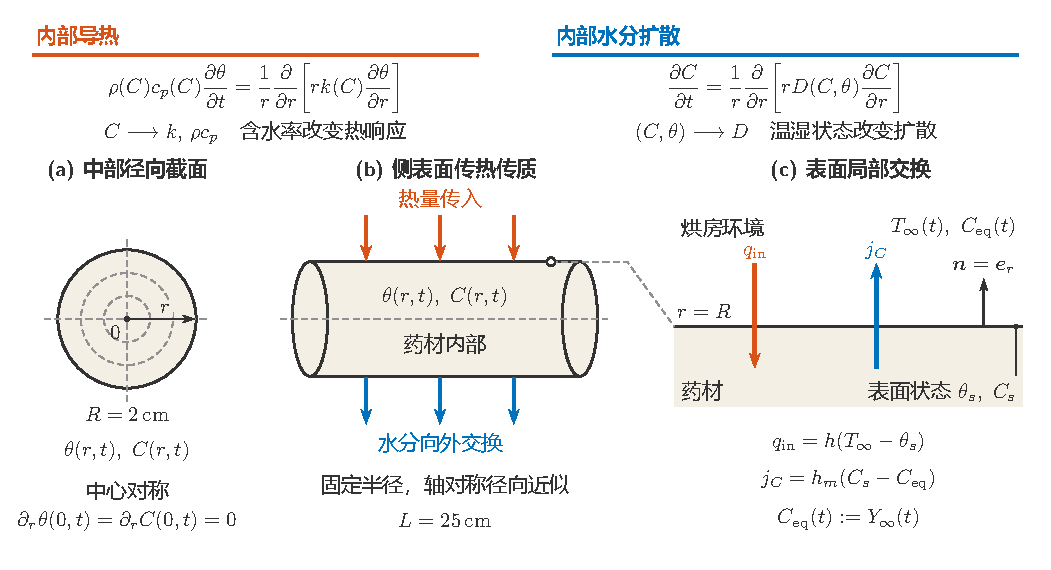
\includegraphics[width=\linewidth]{fig_mechanism_q2_q3.pdf}
\caption{固定半径下药材的径向传热传质与局部物性耦合示意}
\label{fig:mechanism}
\smallskip
\begin{minipage}{\linewidth}
\small 图中几何未按比例绘制，同心虚线仅表示径向位置。箭头示意 $T_\infty>\theta_s$、$C_s>C_{\rm eq}$ 时的传递方向；$q_{\rm in}$ 取热量传入为正，$j_C$ 取含水率向外交换为正。$C$ 为干基含水率，$j_C$ 对应本模型的含水率扩散通量。等效边界输入采用 $C_{\rm eq}:=Y_\infty$。本图适用于问题二、三的固定半径模型。
\end{minipage}
\end{figure}
\end{document}
